% This file was created with tikzplotlib v0.10.1.
% This file was created with tikzplotlib v0.10.1.
\definecolor{mycolor1}{rgb}{0.00000,0.44700,0.74100}%
\definecolor{mycolor2}{rgb}{0.85000,0.32500,0.09800}%
\definecolor{mycolor3}{rgb}{0.92900,0.69400,0.12500}%
\definecolor{mycolor4}{rgb}{0.49400,0.18400,0.55600}%

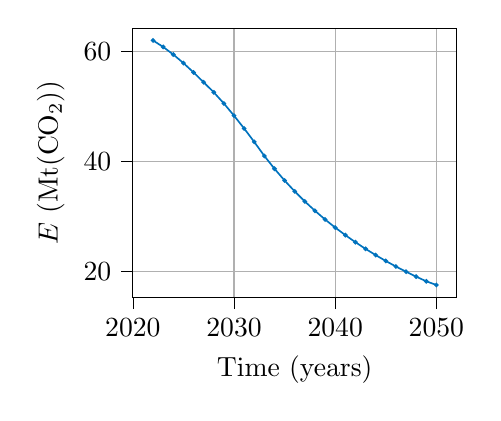
\begin{tikzpicture}

\definecolor{darkgray176}{RGB}{176,176,176}
\definecolor{forestgreen4416044}{RGB}{44,160,44}
\definecolor{lightgray204}{RGB}{204,204,204}

\begin{axis}[
scale = 0.6,
/pgf/number format/1000 sep={},
legend cell align={left},
legend style={fill opacity=0.8, draw opacity=1, text opacity=1, draw=none},
tick align=outside,
tick pos=left,
x grid style={darkgray176},
xlabel={Time (years)},
xmajorgrids,
xmin=2020, xmax=2052,
xtick style={color=black},
y grid style={darkgray176},
ylabel={\(\displaystyle E\) (Mt(CO$_2$))},
ymajorgrids,
ymin=15.3198142436275, ymax=64.2239963012035,
ytick style={color=black}
]
\addplot [semithick, mycolor1, mark=*, mark size=.5, mark options={solid}]
table {%
2022 62.00107893495
2023 60.8167620840584
2024 59.4444586794777
2025 57.8890255459168
2026 56.1877183173264
2027 54.3975171304688
2028 52.5684883062002
2029 50.5450668039021
2030 48.3258611776969
2031 45.9974738999893
2032 43.552106704227
2033 41.0011109775708
2034 38.6712001993099
2035 36.5313827824879
2036 34.5574632934714
2037 32.7301516680728
2038 31.0336627490733
2039 29.4547621227277
2040 27.9821336794484
2041 26.6059580085492
2042 25.317623626056
2043 24.1095211954216
2044 22.9748902623482
2045 21.9077001835989
2046 20.9025542398414
2047 19.9546102274829
2048 19.0595133408377
2049 18.2133386302398
2050 17.5427316098809
};
% \addlegendentry{Simple}
\end{axis}

\end{tikzpicture}
